\smallframetitle

\section{From 08/07/24 to 12/07/24}
\insertsectionframe

\subsection{further advancement on road detection}
\insertsubsectionframe

\begin{frame}{Little advancement}
    \begin{block}{City name detection}
        For each city detected, we find the closest base station to the center of the said city. 
        We then declare that the name of the city is the value contained in the field "nom\_com" of the base station.
    \end{block}

    \begin{figure}
        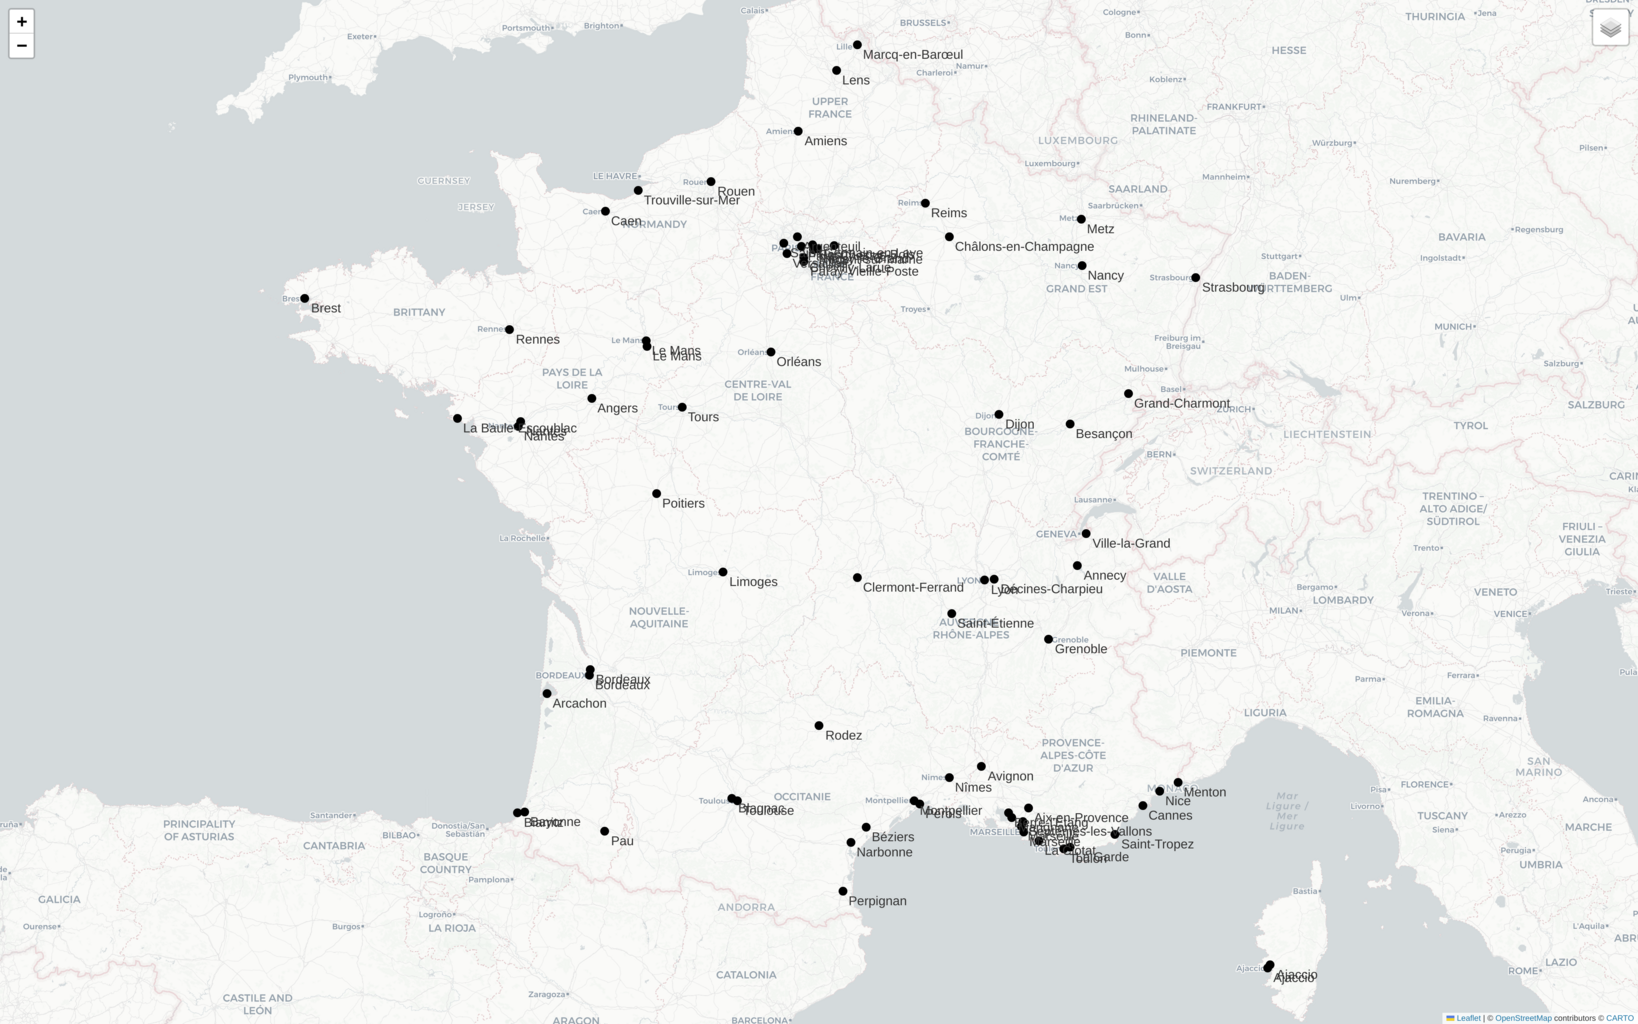
\includegraphics[height=0.4\paperheight]{images/road_detection/cities_centers_with_name.png}
        \caption{Cities centers with name}
    \end{figure}
\end{frame}

\begin{frame}{New method (1/2)}
    \begin{block}{Edges weight}
        For each couple of cities, we compute a weight using this formula :
        $$w_{\text{city1, city2}} = \frac{\min(\text{size(city1)},\text{size(city2)})}{\text{dist(city1, city2)}}$$
        With the size of a city refering to the number of base stations detected inside that city.
        
        We the keep all the edges whose weight is superior to a certain value.
    \end{block}

    \begin{figure}
        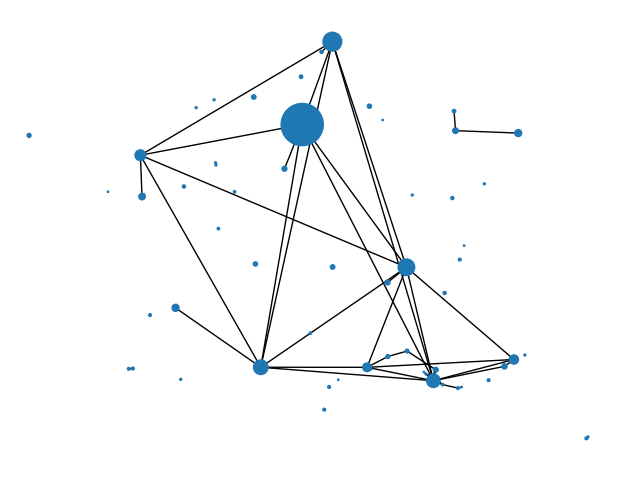
\includegraphics[height=0.3\paperheight]{images/road_detection/edges_weight_filtration.png}
        \caption{weight filtration, cap value = $0.1$}
    \end{figure}
\end{frame} 

\begin{frame}{New method (2/2)}
    \begin{block}{Edges weight}
        We then apply the angle criterion to the resulting graph
    \end{block}

    \begin{figure}
        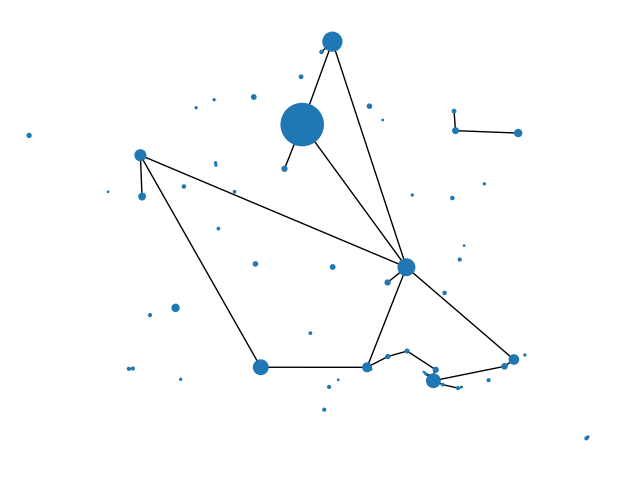
\includegraphics[height=0.4\paperheight]{images/road_detection/edges_weight_angle_filtration.png}
        \caption{weight and angle filtration, cap value = $0.1$, angle value = $15$ degrees}
    \end{figure}
\end{frame} 